\section{Comparing \acs{RS} Scheme Strengths}

Our first idea was to keep a constant data size of $k=80$ and add parity bytes, making the entire message longer.
However, longer packets require more energy to transmit, a metric which has to be included somehow when comparing different $k$.
Furthermore, because of the size limit of the \ac{MPDU} of 127 bytes, of which 26 are already used, this only leaves $n=101$ bytes with a maximum of $n-k=19$ parity bytes, which would not allow to encode with more than 18\% coding overhead.
We could have split the message into two packets, however, this would have made it even harder to compare them, since now two packets must be received in the right sequence.

Therefore, we abandoned this idea and fit the entire encoded message into 80 bytes, including parity bytes as shown in Figure~\ref{fig:rs_codeword}.
This means we can only transfer $k$ bytes of encoded data, effectively reducing data rate while gaining robustness, which we want to use for a metric for comparing \ac{RS} performance.
We combine this reduction of data rate and the corruption of decoded packets as throughput, normalized over the number of \emph{received} messages.
We calculated the normalized throughput $T(80, k)$ using the following formula:

\[ T(80, k) = \frac{k}{80} \frac{PRR_{decoded}}{PRR_{received}} \]

This metric allows us to compare \ac{RS} performance not only between different coding strengths, but augment that comparison with context of the link's quality.
% The normalized throughputs of the original versus simulated links are also available in Figures~\ref{fig:prr_link_01_fec} and \ref{fig:prr_link_10_fec}.
% Especially the drop in Figure~\ref{fig:prr_link_01_receiver} visualizes the previous findings that the simulation slightly underestimates, but never overestimates \ac{RS} decoded \ac{PRR}.

For each of the four links discussed in Section~\ref{sec:packet_reception_rate} we simulated new $RS(80, k)$ encoded payload for $k$ in 10 byte increments up to $k=60$, then in 2 byte increments up to $k=78$.
We plotted the normalized throughputs $T(80, k)$ in Figure~\ref{fig:throughput_link_fec}, with the dashed line showing throughput without RS encoding.
The graphs illustrate that even using only 2 parity bytes at $k=78$ can already significantly improve \ac{PRR}, since most messages only have a few burst errors, and all those constrained to one byte can be corrected.

Adding two more parity bytes for $k=76$ improves \ac{PRR} even more, but only in a few areas.
From $k=74$ to $k=60$ no significant improvement shows, especially at low temperatures.
Using $k=60$ shows stability up to high temperature of $80\,^{\circ}\mathrm{C}$ in all Figures except \ref{fig:throughput_link_10_receiver_fec}.
At and below $k=50$ no improvement of throughput is visible except in Figure~\ref{fig:throughput_link_10_receiver_fec}, where $k=30$ and $k=20$ hold throughput the longest.

By comparing Figure~\ref{fig:prr_link_01_receiver_fec} and \ref{fig:throughput_link_01_receiver_fec}, we can deduct that in that link the simulated throughput above \SI{70}{\celsius} is actually worse than in reality. Therefore we can safely assume $k=60$ as stable at that temperature.

\begin{figure}[t]
	\subfigure[Simulated link~\ref{fig:prr_link_01_transmitter}.] {
		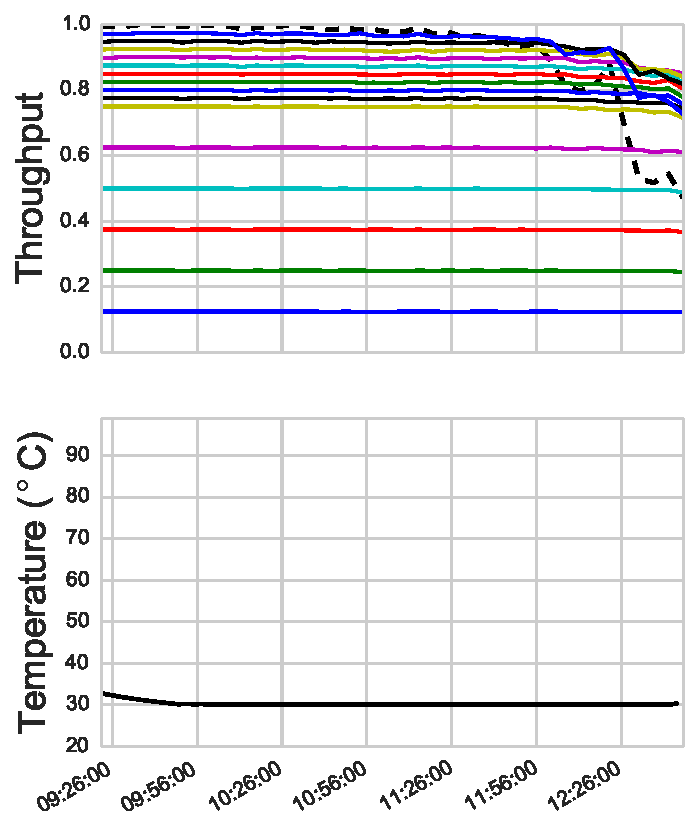
\includegraphics[width=0.475\columnwidth]{figures/fec_scheme_box0_box1_0-1_Throughput}
		\label{fig:throughput_link_01_transmitter_fec}
	}
	\subfigure[Simulated link~\ref{fig:prr_link_01_receiver}.] {
		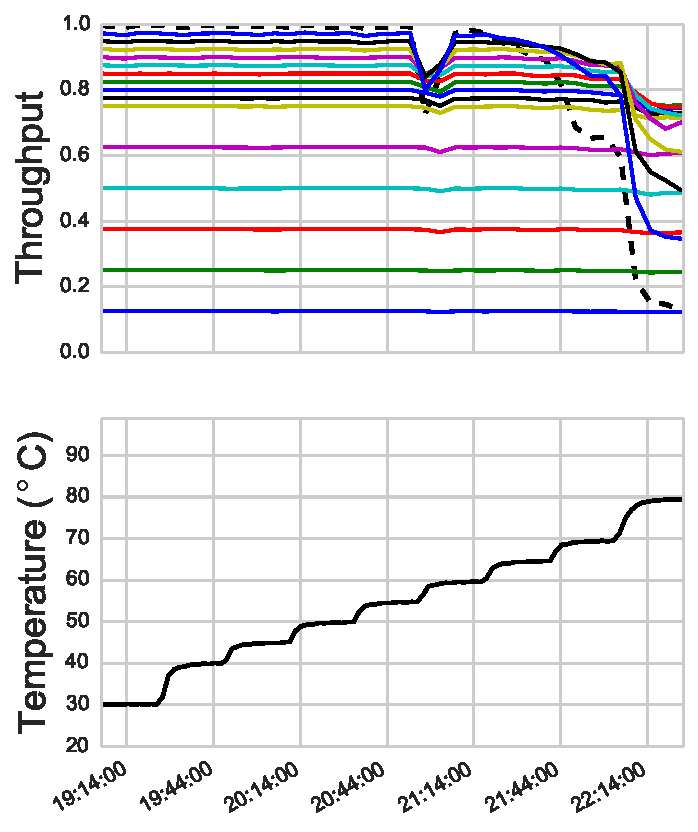
\includegraphics[width=0.475\columnwidth]{figures/fec_scheme_box1_box0_0-1_Throughput}
		\label{fig:throughput_link_01_receiver_fec}
	}
	\subfigure[Simulated link~\ref{fig:prr_link_10_receiver}.] {
		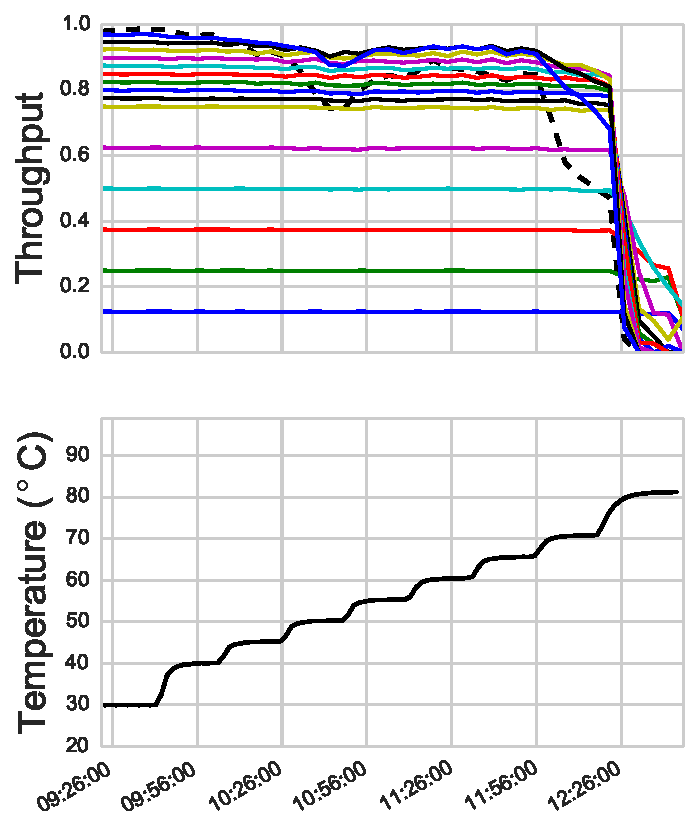
\includegraphics[width=0.475\columnwidth]{figures/fec_scheme_box0_box1_1-0_Throughput}
		\label{fig:throughput_link_10_receiver_fec}
	}
	\subfigure[Simulated link~\ref{fig:prr_link_10_transmitter}.] {
		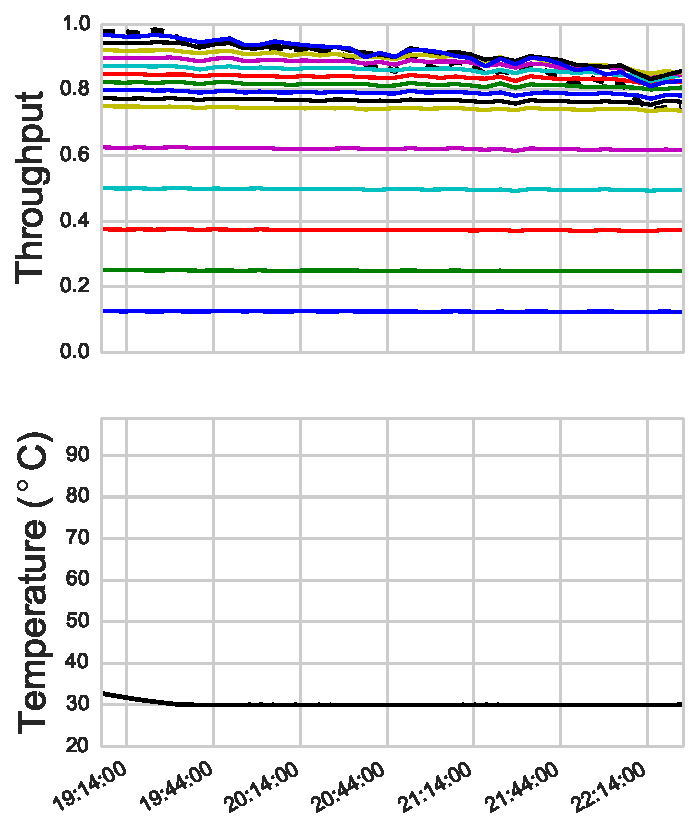
\includegraphics[width=0.475\columnwidth]{figures/fec_scheme_box1_box0_1-0_Throughput}
		\label{fig:throughput_link_10_transmitter_fec}
	}
	\caption{Comparison of throughputs $T(80, k)$ of all four simulated links of Section~\ref{sec:packet_reception_rate} for \\$k \in \{10,20,30,40,50,60,62,64,66,68,70,72,74,76,78\}$ over temperature. The dashed line shows throughput at $k=80$, which is equivalent to using no parity bytes.}
	\label{fig:throughput_link_fec}
\end{figure}

